\section{Introduction}


\begin{figure}[h]
    \centering
    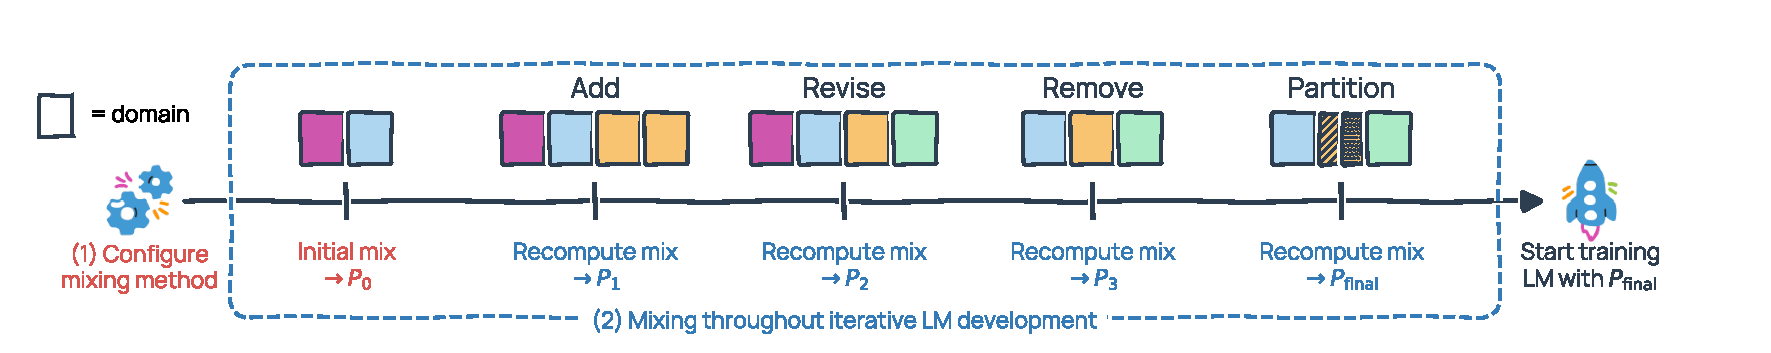
\includegraphics[width=1.0\linewidth, trim=0 0 0 1cm, clip]{figs/fig1_output.pdf}
    \caption{Two problems with data mixing encountered during LM development: (1) How to best configure your mixing method? (2) How to efficiently mix under evolving domain sets?}
    \label{fig:banner}
\end{figure}

Modern language models (LMs) are trained on datasets composed of many domains, such as web text, code, and PDFs. The composition of these domains is crucial for strong downstream performance, making data mixing a first-order component of LM development~\citep{dubey2024llama, qwen2.5, olmo2025olmo3}. 
However, finding a good mix is non-trivial: practitioners often resort to manual weight tuning or exhaustive search, which can require many training runs---possibly thousands of GPU hours---to assess performance.
This has resulted in a growing literature on data mixing methods that aim to find strong mixtures systematically with less compute~\citep{xie2023doremioptimizingdatamixtures, fan2024dogedomainreweightinggeneralization, chen2025aioliunifiedoptimizationframework}. 
Many mixing methods that achieve promising results follow a common \textit{offline mixing schema}~\citep{liu2025rethinkingdatamixturelarge, liu2025regmixdatamixtureregression, ye2025datamixinglawsoptimizing} that consists of three steps: 1. train a set of smaller proxy models on different mixtures (a ``swarm''), 2. fit a regression model on this swarm to predict performance from mixture weights, and 3. propose a final mix that optimizes predicted performance. 

However, data mixing remains far from solved: translating these methods to real-world LM development surfaces challenges that the existing literature does not address.
In this work, we present \olmix, a mixing framework developed for pre-training Olmo~3~\citep{olmo2025olmo3}, a family of fully open, state-of-the-art language and reasoning models at the 7B and 32B parameter scales.
We identify two challenges in applying data mixing methods both at the \emph{start of} LM development--- configuring a mixing method on an initial domain set---and \emph{throughout} development---recomputing mixtures efficiently as domains evolve (Figure~\ref{fig:banner}). \olmix makes progress on addressing both.




\textbf{P1: The mixing configuration problem (\S\ref{sec:config-choices}).} At the start of LM development, we must configure a mixing method on an initial set of domains. However, the configuration space of existing methods is poorly understood; design choices are often unjustified, contradict across methods, or fail to address practical issues like data constraints (Table~\ref{tab:mixing_design_choices}). 
As a result, practitioners have conflicting or little guidance on which choices lead to a strong mixing method.


The first component of \olmix addresses P1 through a comprehensive study of the configuration space of the offline mixing schema. 
We identify seven key design choices needed to instantiate a mixing method from the schema, and we empirically study each design choice in the context of pre-training Olmo 3. Below, we highlight several of these design choices and our findings:
\begin{enumerate}[itemsep=0pt, topsep=2pt, leftmargin=12pt]
    \item \emph{What is the minimum number of proxy runs (swarm size) needed to learn an effective mix for a given domain set?} 
    We find that the required number of runs scales linearly with the number of domains (Figure~\ref{fig:swarm_size}).

    \item \emph{Is there an optimal family of regression models for predicting mix performance?}
    We find that different regression model families excel at different swarm sizes---a key confounding factor that explains disagreement in prior work---but that the log-linear model adapted from~\citet{ye2025datamixinglawsoptimizing} achieves the best overall downstream performance (Figure~\ref{fig:regression_models}).   
        
    \item \emph{How can we perform data mixing under finite data constraints?} Existing methods assume unlimited data, but in practice, certain mixes require sampling more data than is available, leading to excessive sample repetition that degrades performance~\citep{muennighoff2025scalingdataconstrainedlanguagemodels}. We show that incorporating constraints into the mixture optimization problem controls sample repetition while maintaining performance, and that these constraints significantly shape the proposed mix (Figure~\ref{fig:vary_rep_top_7}).    
\end{enumerate}

These findings inform our base mixing method, \base (Algorithm~\ref{alg:base_method}), which we use throughout Olmo~3 development and as a building block for addressing P2.

\textbf{P2: The evolving domain problem (\S\ref{sec:conditional_mixing}).} 
Existing mixing literature assumes a fixed domain set~\citep{albalak2024surveydataselectionlanguage}, but real-world LM development is iterative. 
In our experience building Olmo 1--3~\citep{olmo2025olmo3}, we repeatedly added, removed, revised, and partitioned datasets---a pattern also observed in other iterative development efforts, such as SmolLM 1--3~\citep{bakouch2025smollm3}.
As a result, mixtures must repeatedly be recomputed in practice as the domain set evolves over time. 
However, recomputing from scratch (e.g., using \base) after each domain update becomes increasingly expensive as practitioners make more updates to their datasets. 
Instead, we propose to leverage information from historical mixtures, motivating a new problem: \emph{given an existing mix, how do we efficiently recompute the mix to maintain strong performance after a domain update?} 


The second component of \olmix addresses P2 by introducing a spectrum of recomputation strategies that trade off compute cost against performance. At one end is full recomputation---mixing from scratch after each domain update---which achieves high performance but incurs high computational cost. We make the following contributions developing \textit{mixture reuse} alternatives along this performance-cost spectrum (Figure~\ref{fig:mixreuse}):
\begin{enumerate}[itemsep=0.00pt,topsep=0pt,leftmargin=12pt]
\item We propose \fullmixreuse, a mechanism that reuses the existing mix over the domains that are unaffected by the update. In particular, this mechanism freezes the relative weights among the unaffected domains and recomputes only their total weight alongside the weights of the affected domains. This restricts recomputation (via \base) to a lower-dimensional subspace, reducing computational cost.
\item We analyze when \fullmixreuse performs as well as full recomputation. The performance gap is governed by how much the optimal ratios change after the update and the coupling between reused and recomputed domains, measured by how much they impact the same downstream tasks. 
When both effects are small, \fullmixreuse roughly matches full recomputation while being less costly.
\item We propose \partialmixreuse, an extension of \fullmixreuse that provides a middle ground between full reuse and full recomputation which selectively recomputes the mix on some unaffected domains in addition to the affected ones. This approach can reduce coupling effects and narrow the performance gap to full recomputation at a slightly higher cost than \fullmixreuse.
\end{enumerate}
 
Empirically, we evaluate \olmix---combining our configuration from P1 (\base) with our reuse mechanisms from P2 (\fullmixreuse and \partialmixreuse)---in a real-world LM development setting where the domain set evolves through 5 updates culminating in 64 domains.
When training 1B parameter models on 100B tokens, \fullmixreuse improves over the natural distribution (a baseline with ratios proportional to domain sizes) by +11.6\% and captures 95\% of full recomputation's gains while requiring 74\% fewer proxy runs.
\partialmixreuse reaches 98\% (+12.0\% improvement) while using 67\% fewer proxy runs.
In addition, our best mix obtained via mixture reuse is $3.05\times$ more data-efficient than the natural distribution, reaching the same final performance in one-third as many training steps.
